\documentclass[10pt, a4paper]{scrartcl}

\usepackage{vorschule}
\usepackage[
    typ=ab,
    fach=Informatik,
    lerngruppe={Q2},
    nummer={IV.3},
    module={Symbole,Lizenzen},
    seitenzahlen=keine,
    farbig,
    lizenz=cc-by-nc-sa-4,
]{schule}

\usepackage[
	kuerzel=Ngb,
	reihe={Nichtlineare Datenstrukturen: Bäume},
	version={2020-09-16},
]{ngbschule}

\author{J. Neugebauer}
\title{Der ID3-Algorithmus}
\date{\Heute}

\setzeAufgabentemplate{ngbnormal}


\begin{document}

\ReiheTitel

\begin{rahmen}\small
	\begin{minipage}{0.69\textwidth}
		Die Titanic wurde 1912 gebaut und stach am 14. April zu ihrer Jungfernfahrt in See. An Bord waren über 2200 Passagiere, die sich in drei Klassen zur ersten Überfahrt des Ozeanriesen eingebucht hatten (legal bezahlt oder illegal eingeschmuggelt). Gegen 23:40 Uhr kollidierte die Titanic mit einem Eisberg und sank zwei Stunden und 40 Minuten später vollständig.
		
		Trotz der einigermaßen langen Zeit bis zum Sinken des Schiffes überlebten nur etwa 686 Menschen das Unglück.
	\end{minipage} \hfill
	\begin{minipage}{0.3\textwidth}
		\begin{center}
			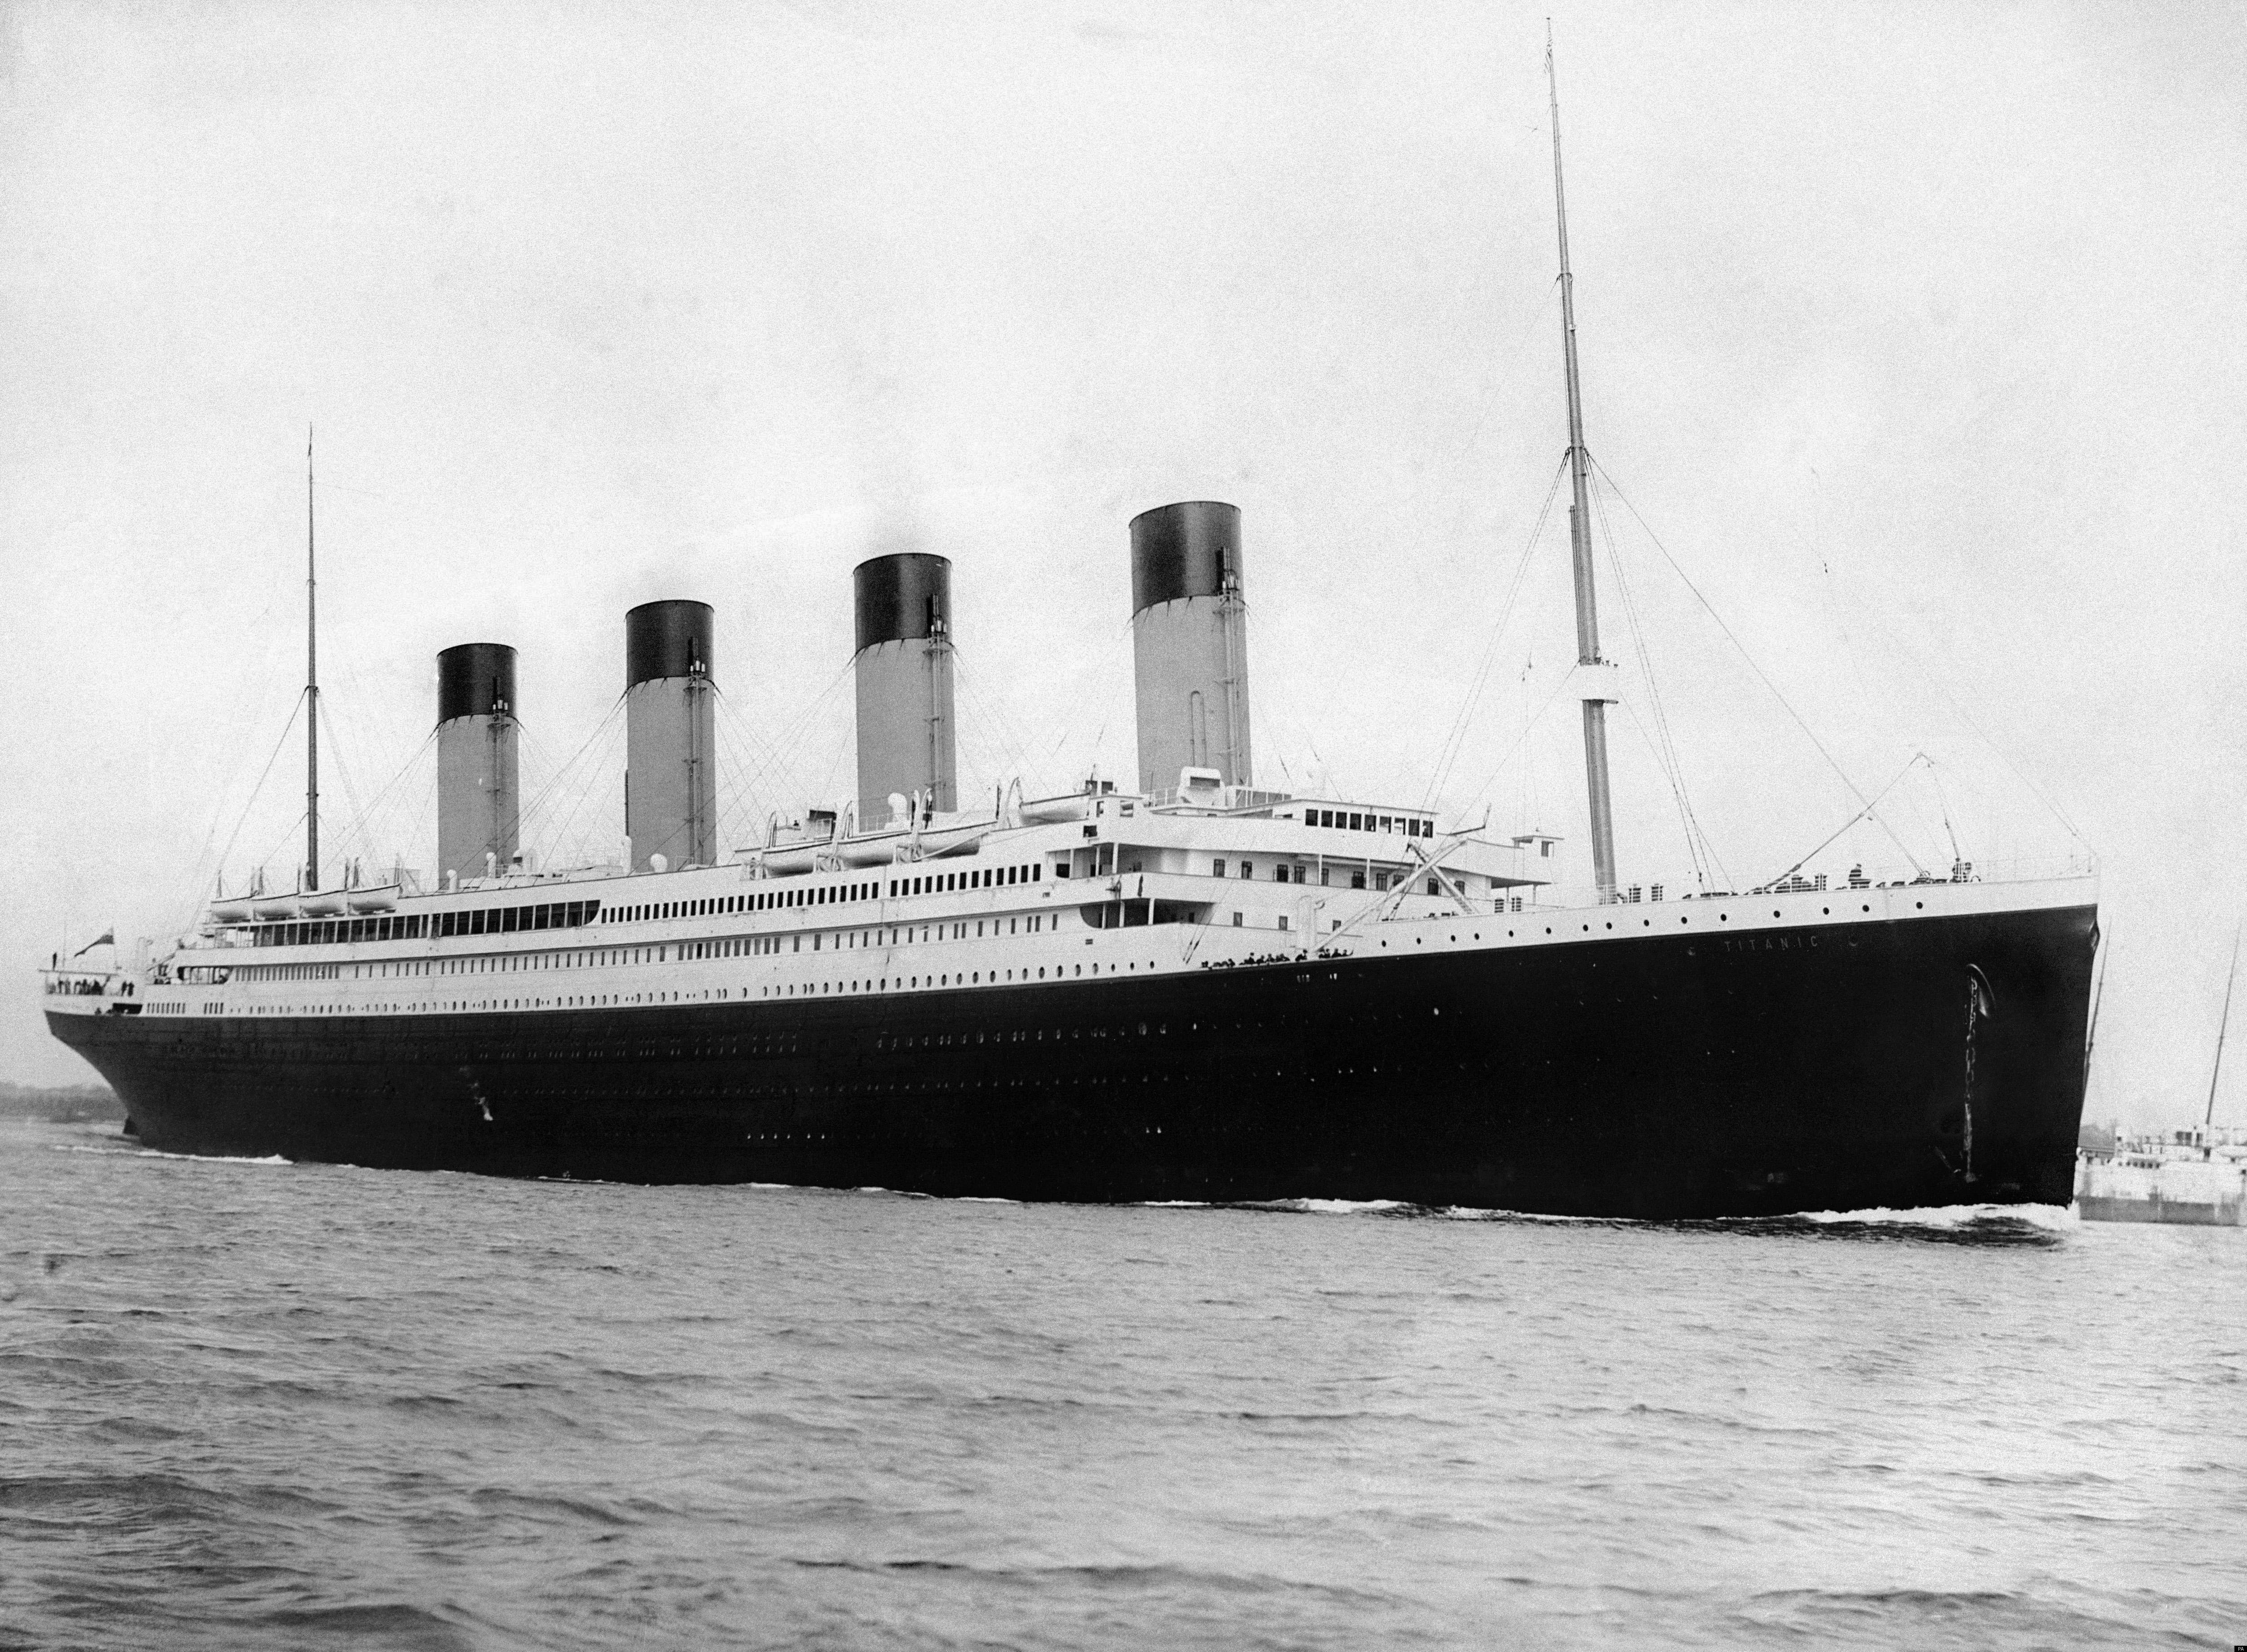
\includegraphics[width=4.5cm]{Q2-AB.3-Abb_RMS Titanic.jpg}
		\end{center}
	\end{minipage}
\end{rahmen}
\bigskip

Der vorliegende Datensatz ist ein bereinigter Auszug aus der Passierliste der Titanic. Wir wollen nun mittels des \emph{ID3-Algorithmus} den Computer einen \emph{Entscheidungsbaum} generieren lassen, der für einen Passagier entscheidet, ob er überlebt hat, oder nicht.

\begin{aufgabe}
	\operator{Berechne} die \emph{Entropie} $E_{gesamt}$ des vollständigen Datensatzes bezüglich des Zielattributes 
	\texttt{survived}.
	
	\begin{center}
		$E_{gesamt} = $\linie[12cm]
	\end{center}
		
	\begin{infobox}
		Die \emph{Entropie} berechnet sich durch $E_{gesamt} = -P_{ja}\cdot \log_2{(P_{ja})} -P_{nein}\cdot \log_2{(P_{nein})}$, wobei $P_{ja/nein}$ den Anteil der Datensätze mit der Ausprägung \enquote{überlebt = ja} bzw. \enquote{überlebt = nein} darstellt.
	\end{infobox}
\end{aufgabe}

\begin{aufgabe}
	\operator{Berechne} die \emph{Entropie} für alle Ausprägungen (Werte) des Attributes \linie[4cm] bezüglich des Zielattributes \texttt{survived}.
	
	\begin{center}
		$E_{\hspace{2cm}} = $\linie[12cm]\\[.4cm]
		$E_{\hspace{2cm}} = $\linie[12cm]\\[.4cm]
		$E_{\hspace{2cm}} = $\linie[12cm]
	\end{center}
	
	\begin{infobox}
		Die \emph{Entropie} $E_{Attributswert}$ berechnet sich wie oben, allerdings werden nur Zeilen berücksichtigt, bei denen das betreffende Attribut den betreffenden Wert hat (z.B. alle Zeilen bei denen \enquote{sex = male} gilt).
	\end{infobox}
\end{aufgabe}

\begin{aufgabe}
	\operator{Berechne} den \emph{Informationsgewinn} für dein Attribut.
	
	\begin{center}
		$IG_{\hspace{2cm}} = $\linie[12cm]
	\end{center}
	
	\begin{infobox}
		Der \emph{Informationsgewinn} $IG_{Attribut}$ eines Attributs berechnet sich durch $E_{gesamt} - \sum{P_{Attributwert}\cdot E_{Attributwert}}$.
	\end{infobox}
\end{aufgabe}

\end{document}
